\documentclass[UTF8,11pt,a4paper]{ctexart}
\usepackage[margin=2.1cm]{geometry}
\usepackage{amsmath,amssymb,booktabs,graphicx,float,hyperref,fancyhdr}
\hypersetup{colorlinks=true,linkcolor=black,citecolor=black,urlcolor=blue!55!black}
\setlength{\parindent}{2em}
\setlength{\parskip}{0.15em}
\pagestyle{fancy}
\setlength{\headheight}{14pt}
\fancyhf{}
\fancyhead[C]{2025 MCM Problem C：最小提示消融基线}
\fancyfoot[C]{\thepage}

\title{2028 年奥运奖牌榜预测与影响因素分析}
\author{同模型最小提示消融基线}
\date{2026 年 8 月}

\begin{document}
\maketitle

\begin{abstract}
本文针对 2028 年奥运会奖牌榜预测问题，综合运用随机森林、Logistic 回归、滚动验证和情景分析等方法进行研究。首先对奖牌、运动员、主办国和比赛项目数据进行清洗，并对国家名称进行统一。其次，建立东道主修正基线与随机森林组合模型，预测各国总奖牌数和金牌数。模型预测美国将获得约 124.27 枚奖牌，其中金牌 43.79 枚；中国将获得约 88.47 枚奖牌，其中金牌 38.86 枚。然后，利用 Logistic 回归预测从未获牌国家在 2028 年获得首枚奖牌的概率，预计首牌国家数为 5.08 个，90\% 计数区间为 2--9 个。最后，通过项目奖牌份额和国家--项目残差分析比赛项目及教练可能产生的影响，并提出德国田径、西班牙水上项目和埃及击剑三个投资方向。滚动验证结果表明，总牌和金牌模型的平均绝对误差分别为 1.441 和 0.627，说明模型具有一定预测能力。

\noindent\textbf{关键词：}奥运会；奖牌预测；随机森林；Logistic 回归；滚动验证
\end{abstract}

\tableofcontents
\newpage

\section{问题重述}

题目要求根据历届奥运会奖牌榜、运动员、主办国和比赛项目数据，对 2028 年洛杉矶奥运会奖牌情况进行预测。主要任务包括：预测各国金牌数和总奖牌数并给出不确定性；分析可能首次获得奖牌的国家；讨论比赛项目设置对不同国家的影响；研究“伟大教练效应”并给出投资建议。

\section{问题分析}

该问题属于多源历史数据预测问题。奖牌数与上一届成绩、参赛规模、项目覆盖度和东道主身份有关，因此可建立监督学习模型。对于从未获牌国家，需要将问题转化为二分类问题。比赛项目的变化可通过各国在不同项目中的历史奖牌份额进行分析。教练效应无法直接观测，可通过国家在某项目上的异常增长进行间接识别。

在数据处理中，运动员表的团队项目会将一枚奖牌记录在多名运动员名下，因此国家奖牌目标采用官方奖牌表，运动员表用于提取参赛人数和项目特征。由于本地项目表只提供到 2024 年，2028 年预测暂时沿用 2024 年项目结构，并将新增项目单独作为情景处理。

\section{模型假设}

\begin{enumerate}
\item 历史数据能够反映各国竞技水平的变化趋势；
\item 2028 年基准项目结构与 2024 年相同；
\item 东道主身份会对奖牌数产生正向影响；
\item 短期内各国参赛规模不会发生极端变化；
\item 国家--项目的连续正残差可作为教练效应的候选信号。
\end{enumerate}

\section{数据预处理}

首先统一历届国家名称与 NOC 代码，并删除特殊代表团。其次，以官方奖牌表作为国家级预测目标，避免团队项目重复计数。然后，从运动员数据中构造参赛人数、覆盖项目数、参赛小项数和累计参赛届数等特征。对项目数据中的缺失符号进行处理，并计算各项目在 2016--2024 年的奖牌份额。

\section{奖牌预测模型}

\subsection{特征构造}

设国家 $i$ 在第 $t$ 届的奖牌数为 $Y_{i,t}$。选取上一届奖牌数、近三届加权奖牌数、奖牌变化量、参赛人数、项目数、小项数、累计参赛届数和东道主变量等特征，记为向量 $\boldsymbol{x}_{i,t}$。

\subsection{组合预测模型}

首先建立包含东道主修正的历史基线 $B_{i,t}$，再训练随机森林模型 $F(\boldsymbol{x}_{i,t})$。最终预测为
\begin{equation}
\widehat{Y}_{i,t}=0.5B_{i,t}+0.5F(\boldsymbol{x}_{i,t}).
\end{equation}
该方法既保留上一届成绩信息，又利用随机森林拟合非线性关系。总牌和金牌分别建模，并将预测结果缩放到 1039 枚总牌和 328 枚金牌，同时保证金牌数不超过总牌数。

\subsection{滚动验证}

采用 2008、2012、2016、2020 和 2024 年作为验证届次，每次只使用此前数据训练。组合模型的总牌 MAE 为 1.441，金牌 MAE 为 0.627，均优于单独随机森林。

\begin{figure}[H]
\centering
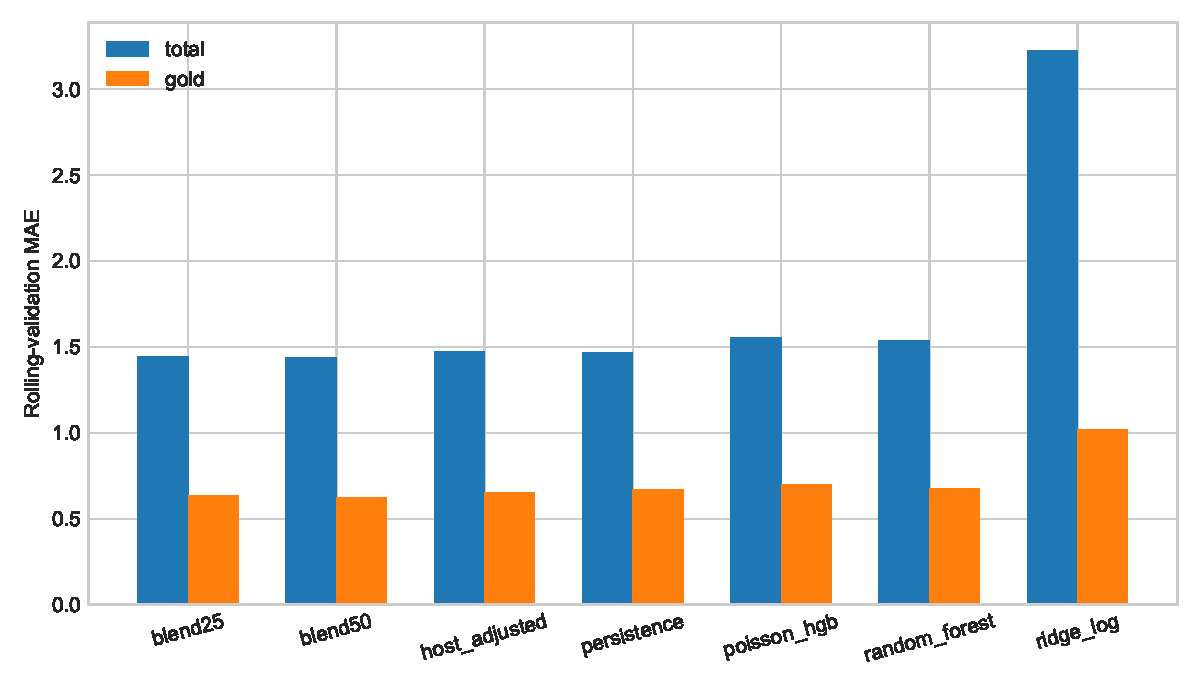
\includegraphics[width=0.78\textwidth]{figures/validation_mae.pdf}
\caption{不同模型的滚动验证 MAE}
\end{figure}

\section{2028 年奖牌预测结果}

表\ref{tab:baseline-forecast}给出部分主要国家的预测结果。美国和中国仍处于领先位置，日本、澳大利亚、英国和法国处于第二梯队。由于误差区间存在较多重叠，预测结果主要用于判断总体趋势。

\begin{table}[H]
\centering
\caption{2028 年主要国家奖牌预测}
\label{tab:baseline-forecast}
\begin{tabular}{lrrrr}
\toprule
国家 & 总牌预测 & 总牌区间 & 金牌预测 & 金牌区间\\
\midrule
美国 & 124.27 & 113.46--137.32 & 43.79 & 33.02--56.79\\
中国 & 88.47 & 77.66--101.52 & 38.86 & 28.08--51.86\\
英国 & 59.05 & 48.24--72.10 & 15.65 & 4.87--28.65\\
法国 & 54.30 & 43.49--67.35 & 13.46 & 2.69--26.46\\
澳大利亚 & 51.41 & 40.60--64.46 & 17.40 & 6.62--30.40\\
日本 & 47.44 & 36.63--60.49 & 18.01 & 7.24--31.01\\
德国 & 36.76 & 25.95--49.81 & 12.04 & 1.27--25.04\\
加拿大 & 31.73 & 20.91--44.78 & 9.17 & 4.95--14.20\\
\bottomrule
\end{tabular}
\end{table}

美国具有东道主优势，因此金牌数预计增加。法国在 2024 年主场效应消失后，奖牌数可能下降。中国整体实力稳定，仍将保持较高金牌数。德国、加拿大和日本的总牌数可能出现一定增长。

\section{首枚奖牌预测}

对于预测时点以前从未获得奖牌且实际参赛的国家，建立 Logistic 回归模型：
\begin{equation}
\operatorname{logit}(p_{i,t})=\beta_0+\beta_1A_{i,t-1}+\beta_2S_{i,t-1}
+\beta_3E_{i,t-1}+\beta_4D_{i,t},
\end{equation}
其中 $A$、$S$、$E$ 和 $D$ 分别表示参赛人数、项目数、小项数和参赛届数。对类别不平衡进行处理，并根据历史首牌率校准概率。通过 50000 次蒙特卡罗模拟，得到 2028 年首牌国家数期望为 5.08，90\% 计数区间为 2--9 个。黎巴嫩、南苏丹、巴勒斯坦、马绍尔群岛和安哥拉的概率较高。

\begin{figure}[H]
\centering
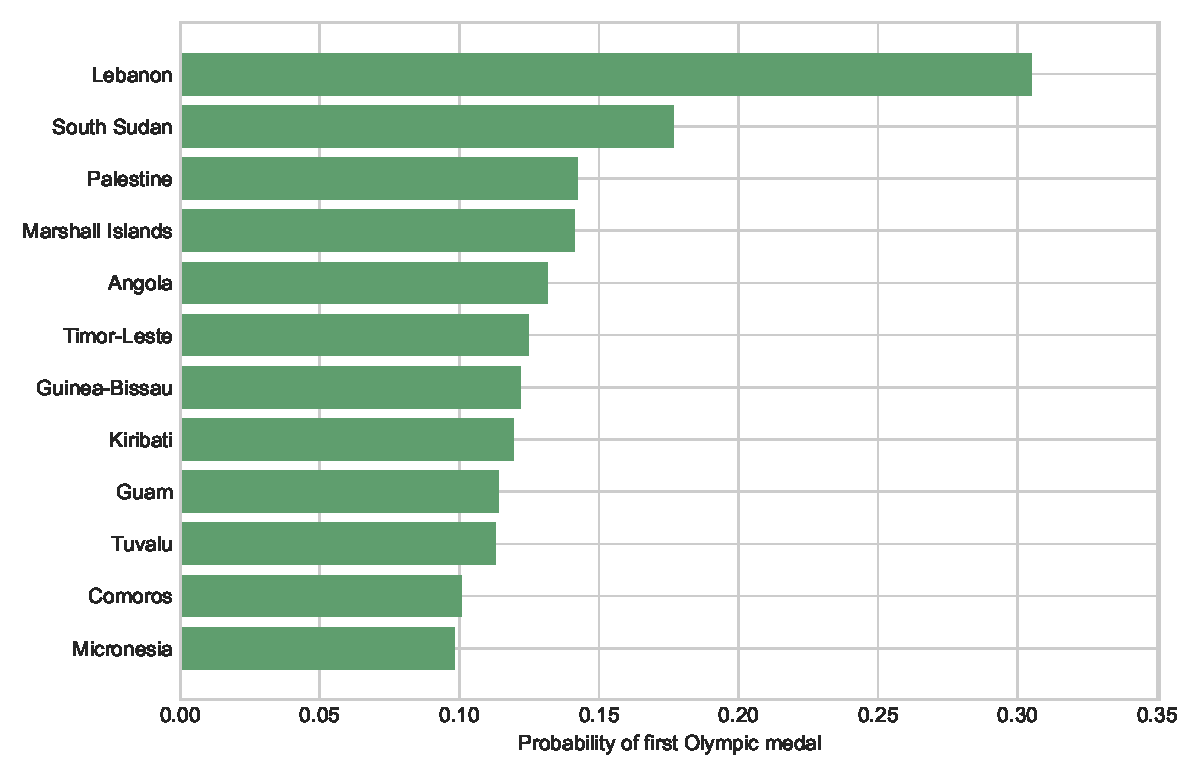
\includegraphics[width=0.76\textwidth]{figures/first_medal_probabilities.pdf}
\caption{首枚奖牌概率较高的国家}
\end{figure}

\section{项目设置影响}

设国家 $i$ 在项目 $s$ 的近三届奖牌数为 $M_{i,s}$，则该国在项目中的奖牌份额为
\begin{equation}
w_{i,s}=\frac{M_{i,s}}{\sum_jM_{j,s}}.
\end{equation}
当项目增加一个小项时，近似新增三枚奖牌，国家 $i$ 的边际增量为 $3w_{i,s}$。计算结果表明，乒乓球新增小项对中国较有利，滑板新增小项对日本较有利，铁人三项新增小项对英国较有利。美国在多个项目上均有优势，因此对单个项目变化的依赖相对较低。

\section{教练效应与投资建议}

附件中没有教练姓名和任职年份，因此不能直接建立教练变量。本文使用国家--项目奖牌预测残差寻找连续两届表现超出预期的项目。中国体操、英国自行车和荷兰田径等项目出现了较明显的持续正残差，可作为教练效应候选。

进一步计算各国项目奖牌转化率与同项目上四分位的差距，得到表\ref{tab:baseline-coach}所示的投资建议。

\begin{table}[H]
\centering
\caption{项目投资建议}
\label{tab:baseline-coach}
\begin{tabular}{llr}
\toprule
国家 & 项目 & 估计增量/枚\\
\midrule
德国 & 田径 & 4.10\\
西班牙 & 水上项目 & 4.07\\
埃及 & 击剑 & 3.56\\
\bottomrule
\end{tabular}
\end{table}

这些国家在相应项目上具有一定参赛基础，但奖牌转化率仍有提升空间。因此可以通过引进高水平教练、优化训练方法和加强重点小项投入来提高成绩。由于缺少教练履历数据，上述结果只表示潜在提升空间。

\section{模型评价}

本文模型具有以下优点：一是综合考虑历史成绩、参赛规模、项目结构和东道主效应；二是采用滚动验证避免使用未来信息；三是给出了预测区间和情景分析。模型也存在不足：2028 年正式项目数据缺失；随机森林解释性有限；教练效应缺少直接数据；首牌国家样本数量较少。未来可加入经济投入、人口、运动员年龄和教练履历等变量，并采用更多模型进行比较。

\section{结论}

本文建立组合模型预测 2028 年奥运奖牌榜。结果显示，美国和中国仍将位于前列，法国可能因失去主场优势而回落。预计约有 5.08 个国家首次获得奥运奖牌。比赛项目变化会对具有传统优势的国家产生更大影响。德国田径、西班牙水上项目和埃及击剑具有较大的潜在提升空间。模型总体预测误差较小，但仍需要结合 2028 年正式项目表和教练数据进一步修正。

\begin{thebibliography}{9}
\bibitem{comap} COMAP. 2025 MCM Problem C: Models for Olympic Medal Tables, 2025.
\bibitem{rf} Breiman L. Random Forests. \emph{Machine Learning}, 2001, 45: 5--32.
\bibitem{logit} Hosmer D W, Lemeshow S, Sturdivant R X. \emph{Applied Logistic Regression}. Wiley, 2013.
\end{thebibliography}

\end{document}
